\documentclass[aspectratio=43,11pt]{beamer}

% ================================================================
% Presentación de TP4 — Dinámica Molecular Regida por el Paso
% Temporal (72.25, ITBA).
% Estilo heredado de TP3/presentacion/template_presentacion_tp3.tex (D27).
% Compilar con: latexmk -pdf presentacion_imagen.tex
% Símbolos nuevos: definir en texto + marca visual la primera vez (ver DEFINICIONES.md §5).
% ================================================================

% ----------------------------------------------------------------
% REVISAR A MANO antes de aceptar (corrección real de TP2: un label
% de eje sobrecargado "suena a eje nombrado por la IA"). Convención
% acordada para TODAS las figuras de esta presentación:
%   eje temporal .......... t [s]
%   paso temporal ......... Δt [s]
%   error cuadrático medio  ECM
%   energía relativa ...... E/E₀
%   error de energía ...... ε_E
%   cantidad de partículas  N
%   fracción usada ........ F_u
%   tiempo al 90% ......... ⟨t₉₀⟩ [s]
%   rapidez ............... v [m/s], f(v)
%   densidad .............. ρ [m⁻²]
% Nada de paréntesis explicativos ni unidades del modelo entre
% corchetes. Si un label no entra en dos o tres símbolos, está mal.
%
% TAMAÑO DE FUENTE (corrección real de TP2: "los tamaños de fuente de
% las figuras son ilegibles"): la letra dentro de cada figura tiene que
% ser comparable a la del resto de la diapositiva. Si no se lee
% proyectada, está mal, sea cual sea el tamaño en puntos.
%
% NUNCA un título adentro del área graficada: eso va en el
% \frametitle. Los parámetros fijos van en el \parambox del costado,
% nunca repetidos en cada entrada de leyenda.
%
% TEXTO (D27): lo escribe una persona a partir de la figura. Los
% títulos de cada diapositiva son provisorios; los recuadros grises con
% "Sxx — ..." marcan qué va (DEFINICIONES.md §3) y se reemplazan.
% ----------------------------------------------------------------

\usepackage[T1]{fontenc}
% "provide=*" permite compilar también en instalaciones mínimas de TeX Live.
\usepackage[provide=*,spanish]{babel}
\usepackage{lmodern}
\usepackage{amsmath,amssymb,bm}
\usepackage{graphicx}
\usepackage{tikz}
\usetikzlibrary{arrows.meta,calc,positioning,decorations.pathmorphing}
% Para controlar leftmargin/itemsep/topsep del itemize angosto de \parambox
% (0.27\textwidth) -- el itemize default de beamer queda con demasiado
% margen y espaciado para una caja tan chica.
\usepackage{enumitem}
% enumitem reemplaza el símbolo de beamer por uno vacío: sin esto los itemize
% sin label explícito (ej. Conclusiones) salen sin viñeta.
\setlist[itemize]{label=\textcolor{TPBlue}{$\bullet$}}

% ---------- Colores ----------
\definecolor{TPBlue}{HTML}{3939B5}
\definecolor{TPBlueDark}{HTML}{29298A}
\definecolor{TPBlack}{HTML}{050505}
\definecolor{TPNavGray}{HTML}{858585}
\definecolor{TPLight}{HTML}{E9E9F2}
\definecolor{TPPlaceholder}{HTML}{F4F4F7}
\definecolor{TPFresca}{HTML}{2E5FD0}
\definecolor{TPUsada}{HTML}{C0392B}

\setbeamercolor{normal text}{fg=black,bg=white}
\setbeamercolor{structure}{fg=TPBlue}
\setbeamercolor{frametitle}{fg=white,bg=TPBlue}
\setbeamercolor{itemize item}{fg=TPBlue}
\setbeamercolor{itemize subitem}{fg=TPBlue}
\setbeamercolor{title box}{fg=white,bg=TPBlue}
\setbeamercolor{databox title}{fg=white,bg=TPBlueDark}
\setbeamercolor{databox body}{fg=black,bg=TPLight}
\setbeamercolor{algorithm box}{fg=black,bg=white}
\setbeamercolor{headline navigation}{fg=TPNavGray,bg=TPBlack}
\setbeamertemplate{items}[circle]
\setbeamertemplate{navigation symbols}{}

\setbeamerfont{frametitle}{size=\Large,series=\mdseries}
\setbeamerfont{normal text}{size=\normalsize}
\setbeamerfont{itemize/enumerate body}{size=\normalsize}
\setbeamerfont{itemize/enumerate subbody}{size=\small}

% ---------- Metadatos ----------
\title{Trabajo Práctico Nro. 4: Dinámica Molecular Regida por el Paso Temporal}
\subtitle{72.25 - Simulación de Sistemas}
\author{%
  Federico Ignacio Ruckauf\texorpdfstring{\textsuperscript{1}}{1}
  \and Federico Spivak Fontaiña\texorpdfstring{\textsuperscript{2}}{2}
  \and Lorenzo Chiossone\texorpdfstring{\textsuperscript{3}}{3}%
}
\institute{Instituto Tecnológico de Buenos Aires}
\date{2026 2C --- Grupo N.º 02}

% URLs de las animaciones (D16). Las de 2.2 (con obstáculos) y 2.3 (sin obstáculos) son las de Lorenzo
% (scripts/sim_gen/generate_animations.sh); la de 2.4 sigue pendiente: reemplazar PENDIENTE al subirla.
\newcommand{\animacionDosCuatroURL}{https://youtu.be/PENDIENTE}
% Videos del Sistema 2: sin obstáculos y con obstáculos, respectivamente.
\newcommand{\animacionSinObstaculosURL}{https://youtu.be/82lP3rStJBo}
\newcommand{\animacionConObstaculosURL}{https://youtu.be/uctSdF2HWXg}

% Si existe logo_itba.png o logo_itba.pdf junto al .tex, se inserta.
\newcommand{\institutionlogo}{%
  \IfFileExists{logo_itba.pdf}{\includegraphics[height=0.75cm]{logo_itba.pdf}}{%
    \IfFileExists{logo_itba.png}{
\includegraphics[height=0.75cm]{logo_itba.png}}{%
      \fbox{\scriptsize LOGO DE LA INSTITUCIÓN}%
    }%
  }%
}

% ---------- Barra superior por sección ----------
% Rangos de diapositivas:
% Introducción 2--4 (incluye Modelo, fusionado -- ver TP2) | Implementación 5--8
% Simulaciones 9--12 | Resultados 13--26 | Conclusiones 27--29
% Anexo 31--32 (apéndice). El cierre (30) queda fuera de la barra.
% Cada rango incluye su \sectiondivider como primera diapositiva del
% bloque. Si se agregan o quitan diapositivas hay que renumerar estos
% rangos a mano.
\newcount\TPNavDot

\newcommand{\navdots}[2]{%
  \begingroup
    \TPNavDot=#1\relax
    \loop
      \ifnum\insertframenumber=\TPNavDot
        \raisebox{0.45mm}{{\color{white}\fontsize{6}{6}\selectfont$\bullet$}}%
      \else
        \raisebox{0.45mm}{{\color{TPNavGray}\fontsize{7}{7}\selectfont$\circ$}}%
      \fi
      \ifnum\TPNavDot<#2\relax
        \kern0.60mm
        \advance\TPNavDot by 1\relax
    \repeat
  \endgroup
}

\newcommand{\navblock}[4]{%
  % #1 ancho, #2 nombre, #3 inicio, #4 fin
  \makebox[#1\paperwidth][c]{%
    \parbox[c][0.62cm][c]{#1\paperwidth}{%
      \centering
      \ifnum\insertframenumber>1
        \ifnum\insertframenumber<#3
          {\color{TPNavGray}\scriptsize\strut #2}%
        \else
          \ifnum\insertframenumber>#4
            {\color{TPNavGray}\scriptsize\strut #2}%
          \else
            {\color{white}\scriptsize\strut #2}%
          \fi
        \fi
      \else
        {\color{TPNavGray}\scriptsize\strut #2}%
      \fi
      \par\vspace{-0.55mm}
      \navdots{#3}{#4}%
    }%
  }%
}

% Fila de navegación por secciones -- factorizada para no duplicarla
% entre las dos ramas de \TPheadline (con y sin franja de relleno).
\newcommand{\TPnavrow}{%
  \makebox[\paperwidth][l]{%
    \navblock{0.16}{Introducción}{2}{4}%
    \navblock{0.18}{Implementación}{5}{8}%
    \navblock{0.16}{Simulaciones}{9}{12}%
    \navblock{0.25}{Resultados}{13}{26}%
    \navblock{0.15}{Conclusiones}{27}{29}%
    \navblock{0.10}{Anexo}{31}{32}%
  }%
}

% La franja azul de relleno (para diapositivas sin título, ej.
% \sectiondivider) NUNCA debe cambiar la altura TOTAL del headline: si se
% suma como una caja extra arriba de la altura de la barra de navegación
% normal, el headline queda 0.05cm (~1.42pt) más alto que en las
% diapositivas con título, y LaTeX no tiene margen para absorberlo en los
% frames centrados verticalmente ([c], o con \vfill como portada/cierre)
% -- produce "Overfull \vbox (1.42271pt too high)" y una línea residual
% visible en el borde superior. Por eso la franja le resta exactamente lo
% mismo que ocupa al "dp" de la barra de navegación (0.28cm -> 0.23cm):
% el total (barra + franja) da siempre 0.78cm, igual que una diapositiva
% con título.
\setbeamertemplate{headline}{%
  \leavevmode
  \ifdefempty{\insertframetitle}{%
    \begin{beamercolorbox}[wd=\paperwidth,ht=0.50cm,dp=0.23cm]{headline navigation}%
      \TPnavrow
    \end{beamercolorbox}%
    \par\nointerlineskip
    \begin{beamercolorbox}[wd=\paperwidth,ht=0.05cm,dp=0cm]{frametitle}\end{beamercolorbox}%
  }{%
    \begin{beamercolorbox}[wd=\paperwidth,ht=0.50cm,dp=0.28cm]{headline navigation}%
      \TPnavrow
    \end{beamercolorbox}%
  }%
}

\setbeamertemplate{frametitle}{%
  \nointerlineskip
  \begin{beamercolorbox}[wd=\paperwidth,ht=0.74cm,dp=0.12cm,leftskip=0.35cm]{frametitle}
    \usebeamerfont{frametitle}\insertframetitle
  \end{beamercolorbox}
}

\setbeamersize{text margin left=0.55cm,text margin right=0.55cm}

% Pie mínimo con número de diapositiva.
\setbeamertemplate{footline}{%
  \leavevmode
  \hbox{\begin{beamercolorbox}[wd=\paperwidth,ht=0.20cm,dp=0.10cm,rightskip=0.18cm]{normal text}
    \hfill{\color{TPNavGray}\tiny\insertframenumber/\inserttotalframenumber}
  \end{beamercolorbox}}
}

% ---------- Componentes reutilizables (heredados de TP2/TP3) ----------
\newcommand{\sectiondivider}[1]{%
  \begin{frame}[c]{}
    \makebox[\linewidth][c]{%
      \begin{beamercolorbox}[wd=0.56\paperwidth,ht=0.55cm,dp=0.15cm,center]{frametitle}
        \large #1
      \end{beamercolorbox}%
    }
  \end{frame}
}

\newcommand{\placeholder}[2][4.4cm]{%
  \begingroup
    \setlength{\fboxsep}{0pt}%
    \setlength{\fboxrule}{0.45pt}%
    \fcolorbox{TPNavGray}{TPPlaceholder}{%
      \parbox[c][\dimexpr#1-2\fboxrule\relax][c]{%
        \dimexpr\linewidth-2\fboxrule\relax}{%
        \centering\color{TPNavGray}\small #2}%
    }%
  \endgroup
}

\newcommand{\maybeimage}[3]{%
  \IfFileExists{#1}{\includegraphics[width=\linewidth,height=#2,keepaspectratio]{#1}}{%
    \placeholder[#2]{#3\\[2mm]\nolinkurl{#1}}%
  }%
}

% Ambas versiones muestran debajo un enlace visible a YouTube.
% En la versión YouTube, además, la propia imagen funciona como enlace.
\newcommand{\videooimagen}[4]{%
  \begin{minipage}{\linewidth}
    \centering
    \ifdefined\versionyoutube
      \href{#3}{\maybeimage{#1}{#2}{#4}}%
    \else
      \maybeimage{#1}{#2}{#4}%
    \fi
    \par\vspace{1mm}
    \href{#3}{{\color{TPBlue}\scriptsize\nolinkurl{#3}}}%
  \end{minipage}%
}

% Caja de parámetros fijos, en la columna derecha (~28% del frame) --
% nunca repetidos dentro de la leyenda (corrección real de TP2). Lista de
% viñetas alineada a la izquierda (no centrada): el contenido se pasa como
% una secuencia de \item, ej. \parambox{\item A \item B \item C}.
\newcommand{\parambox}[1]{%
  \begin{beamercolorbox}[wd=\linewidth,sep=2mm]{databox body}
    \small
    \begin{itemize}[label=\textcolor{TPBlue}{$\bullet$},leftmargin=3.2mm,labelsep=1mm,itemsep=1mm,topsep=0pt,parsep=0pt]
      #1
    \end{itemize}
  \end{beamercolorbox}%
}

% Una animación por diapositiva, con la caja de parámetros al costado.
% #1 imagen, #2 altura, #3 URL, #4 texto del placeholder, #5 parámetros fijos.
\newcommand{\animacionsimple}[5]{%
  \begin{columns}[T,onlytextwidth]
    \begin{column}{0.66\textwidth}
      \videooimagen{#1}{#2}{#3}{#4}%
    \end{column}
    \begin{column}{0.31\textwidth}
      \parambox{#5}%
    \end{column}
  \end{columns}%
}

% Diapositiva de resultados: figura a la izquierda (0.66) y, a la derecha,
% la caja de parámetros fijos y opcionalmente una imagen chica (fotograma
% de la animación o esquema) con su epígrafe.
% #1 figura, #2 altura, #3 texto del placeholder, #4 parámetros fijos,
% #5 imagen chica (vacío = sin imagen), #6 epígrafe de la imagen chica.
% Columnas 0.73 / 0.25 (antes 0.66 / 0.31): la figura queda lo más grande posible y la caja de
% parámetros, en columna a la derecha (pedido del grupo, 23/10).
\newcommand{\resultadofigura}[6]{%
  \begin{columns}[T,onlytextwidth]
    \begin{column}{0.73\textwidth}
      \centering
      \maybeimage{#1}{#2}{#3}%
    \end{column}
    \begin{column}{0.25\textwidth}
      \ifstrempty{#4}{}{\parambox{#4}\par\vspace{2mm}}%
      \ifstrempty{#5}{}{%
        \centering
        \maybeimage{#5}{3.2cm}{Imagen chica}\par
        {\scriptsize\color{TPNavGray}#6\par}%
      }%
    \end{column}
  \end{columns}%
}

\newenvironment{databox}[1]{%
  \begin{beamercolorbox}[wd=\linewidth,sep=1mm,center]{databox title}%
    #1
  \end{beamercolorbox}%
  \par\nointerlineskip
  \begin{beamercolorbox}[wd=\linewidth,sep=2mm]{databox body}%
}{%
  \end{beamercolorbox}%
}

% ================================================================
% PRESENTACIÓN
% Una diapositiva por fila S01--S17 de DEFINICIONES.md §3.
% Figuras: nombres fijos que escriben los scripts de scripts/graph_gen (D28).
% ================================================================
\begin{document}

% 1. PORTADA
\begin{frame}{}
  \vspace{0.35cm}
  \begingroup
    \makebox[\linewidth][c]{%
      \begin{beamercolorbox}[wd=0.91\linewidth,sep=3mm,center]{title box}
        \resizebox{0.92\linewidth}{!}{\strut\inserttitle}\par
        \vspace{1mm}
        {\large\insertsubtitle}
      \end{beamercolorbox}%
    }
    \par
  \endgroup
  \vspace{0.35cm}
  \begin{center}
    {\small\insertauthor\par}
    \vspace{0.18cm}
    {\scriptsize
      \textsuperscript{1}\href{mailto:fruckauf@itba.edu.ar}{fruckauf@itba.edu.ar}\\[0.5mm]
      \textsuperscript{2}\href{mailto:fespivak@itba.edu.ar}{fespivak@itba.edu.ar}\\[0.5mm]
      \textsuperscript{3}\href{mailto:lchiossone@itba.edu.ar}{lchiossone@itba.edu.ar}
      \par
    }
    \vspace{0.13cm}
    {\small\insertinstitute\par}
    \vspace{0.35cm}
    {\large\insertdate\par}
    \vfill
    \institutionlogo
  \end{center}
\end{frame}

% ---------------- INTRODUCCIÓN ----------------
% 2
\sectiondivider{Introducción}

% 3 -- S01 (nada del billar, de obstáculos ni del Sistema 1)
% Formato de «Sistema Real y Objetivo» de TP3: texto a la izquierda, ilustración a la derecha (esquema genérico,
% sin billar ni obstáculos).
\begin{frame}{Introducción}
  \begin{columns}[c,onlytextwidth]
    \begin{column}{0.56\textwidth}
      \begin{itemize}
        \item Partículas que chocan entre sí como resortes lineales
        \item Dinámica molecular por paso temporal: se integran las ecuaciones de Newton con un paso fijo
      \end{itemize}
      \vspace{0.3cm}
      \textbf{Objetivo:} elegir un paso que conserve la energía y comparar el costo con la dinámica dirigida por eventos.
    \end{column}
    \begin{column}{0.41\textwidth}
      \centering
      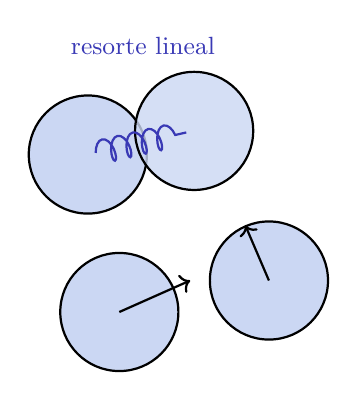
\begin{tikzpicture}[font=\small]
        \draw[thick, fill=TPFresca!25] (0,0) circle (0.75);
        \draw[thick, fill=TPFresca!25, fill opacity=0.8] (1.35,0.3) circle (0.75);
        \draw[decorate, decoration={coil, aspect=0.45, segment length=2mm, amplitude=1.5mm}, thick, TPBlue]
          (0.1,0.02) -- (1.25,0.28);
        \node[TPBlue, above] at (0.7,1.15) {resorte lineal};
        \draw[thick, fill=TPFresca!25] (0.4,-2.0) circle (0.75);
        \draw[->, thick] (0.4,-2.0) -- (1.3,-1.6);
        \draw[thick, fill=TPFresca!25] (2.3,-1.6) circle (0.75);
        \draw[->, thick] (2.3,-1.6) -- (2.0,-0.9);
      \end{tikzpicture}
    \end{column}
  \end{columns}
\end{frame}

% 4 -- S02 (define ξ y E: DEFINICIONES.md §5). Posiciones en negrita; r_i es el radio (R es el del dominio)
\begin{frame}{Modelo}
  \begin{columns}[T,onlytextwidth]
    \begin{column}{0.60\textwidth}
      % Un título por fórmula (pedido del grupo, 23/10); menos aire entre fórmulas para que entren las cuatro
      \setlength{\abovedisplayskip}{3pt}\setlength{\belowdisplayskip}{3pt}
      {\small\textbf{Ecuación de movimiento}}
      \[ m\,\ddot{\mathbf{r}}_i = \mathbf{F}_i = \sum_{j:\,\xi_{ij} > 0} -k\,\xi_{ij}\,\hat{\mathbf{e}}_n \]
      {\small\textbf{Versor normal}}
      \[ \hat{\mathbf{e}}_n = \frac{\mathbf{r}_j - \mathbf{r}_i}{|\mathbf{r}_j - \mathbf{r}_i|} \]
      {\small\textbf{Superposición}}
      \[ \xi_{ij} = r_i + r_j - |\mathbf{r}_j - \mathbf{r}_i| \]
      {\small\textbf{Energía total}}
      \[ E = \sum_i \tfrac{1}{2}\, m\, v_i^2 + \sum_{\text{contactos}} \tfrac{1}{2}\, k\, \xi^2 \]
    \end{column}
    \begin{column}{0.37\textwidth}
      \centering
      % E2: contacto entre dos partículas con la superposición ξ
      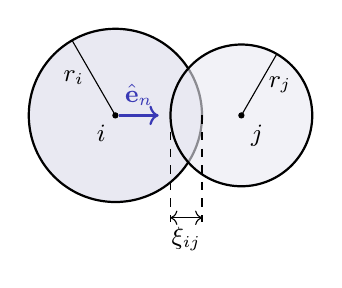
\begin{tikzpicture}[font=\small]
        \draw[thick, fill=TPLight] (0,0) circle (1.1);
        \draw[thick, fill=TPLight, fill opacity=0.6] (1.6,0) circle (0.9);
        \fill (0,0) circle (0.04) (1.6,0) circle (0.04);
        \node[below left] at (0,0) {$i$};
        \node[below right] at (1.6,0) {$j$};
        \draw (0,0) -- node[left] {$r_i$} (120:1.1);
        \draw (1.6,0) -- node[right] {$r_j$} ($(1.6,0)+(60:0.9)$);
        \draw[->, thick, TPBlue] (0.05,0) -- (0.55,0) node[midway, above] {$\hat{\mathbf{e}}_n$};
        \draw[dashed] (0.7,0) -- (0.7,-1.35) (1.1,0) -- (1.1,-1.35);
        \draw[<->] (0.7,-1.3) -- (1.1,-1.3) node[midway, below] {$\xi_{ij}$};
      \end{tikzpicture}
      \par\vspace{2mm}
      {\small $r_i$, $r_j$: radios de partículas}
    \end{column}
  \end{columns}
\end{frame}

% ---------------- IMPLEMENTACIÓN ----------------
% 5
\sectiondivider{Implementación}

% 6 -- Arquitectura del motor, con el estilo del «Diagrama del Motor» de TP3 (sin \resizebox: letra ≥ 10 pt).
% El lazo sigue el orden de BilliardSimulator.run (l.73-115): fuerzas (CIM, obstáculos/usadas, pared) -> Verlet
% -> guardado cada n pasos con v central -> avanzar. Sin símbolos: Δt, Δt₂, x₀, N y t_f se definen después.
% Archivos de salida: io/BilliardFiles.java:24.
\begin{frame}[c]{Arquitectura}
  \centering
  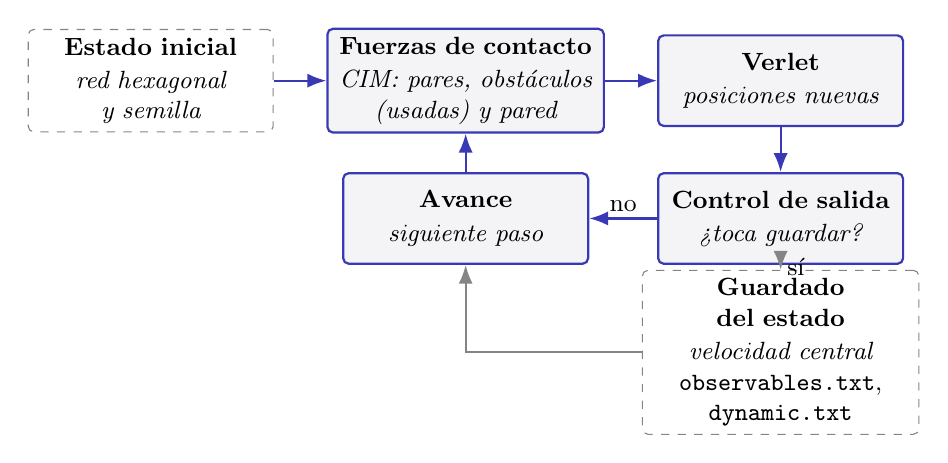
\begin{tikzpicture}[
      caja/.style={rectangle, rounded corners=2pt, draw=TPBlue, thick, fill=TPPlaceholder, align=center,
        minimum height=1.15cm, text width=2.9cm, font=\small, inner sep=3pt,
        execute at begin node=\hyphenpenalty10000\relax},
      externa/.style={rectangle, rounded corners=2pt, draw=TPNavGray, dashed, align=center,
        minimum height=1.15cm, text width=2.9cm, font=\small, inner sep=3pt,
        execute at begin node=\hyphenpenalty10000\relax},
      flecha/.style={-{Latex[length=2.4mm]}, draw=TPBlue, thick},
      flechagris/.style={-{Latex[length=2.4mm]}, draw=TPNavGray, thick},
      etiqueta/.style={font=\small, inner sep=2pt},
    ]
    % Lazo cerrado como en TP3: fuerzas -> Verlet -> ¿guardar? -> avance -> fuerzas; rama gris al guardado
    \node[externa] (ic)  at (0.0,2.1)  {\textbf{Estado inicial}\\[1pt]{\itshape red hexagonal y semilla}};
    \node[caja, text width=3.3cm] (fu) at (4.0,2.1) {\textbf{Fuerzas de contacto}\\[1pt]{\itshape CIM: pares, obstáculos (usadas) y pared}};
    \node[caja]    (ve)  at (8.0,2.1)  {\textbf{Verlet}\\[1pt]{\itshape posiciones nuevas}};
    \node[caja]    (sa)  at (8.0,0.35) {\textbf{Control de salida}\\[1pt]{\itshape ¿toca guardar?}};
    \node[caja]    (av)  at (4.0,0.35) {\textbf{Avance}\\[1pt]{\itshape siguiente paso}};
    \node[externa, text width=3.3cm] (out) at (8.0,-1.35) {\textbf{Guardado del estado}\\[1pt]{\itshape velocidad central}\\\texttt{observables.txt}, \texttt{dynamic.txt}};

    \draw[flecha] (ic) -- (fu);
    \draw[flecha] (fu) -- (ve);
    \draw[flecha] (ve) -- (sa);
    \draw[flecha] (sa) -- node[etiqueta, above] {no} (av);
    \draw[flecha] (av) -- (fu);
    \draw[flechagris] (sa) -- node[etiqueta, right] {sí} (out);
    \draw[flechagris] (out.west) -| (av.south);
  \end{tikzpicture}
  \par\vspace{2mm}
  {\small Misma semilla y configuración $\Rightarrow$ mismo \texttt{observables.txt} (salvo el tiempo de ejecución)}
\end{frame}

% 7 -- S03a (solo Sistema 2: el Sistema 1 va en una sola diapositiva, enunciado; define Δt, Δt₂)
\begin{frame}{Integración: Verlet Original}
  % Un título por fórmula, como en «Modelo»
  \begin{itemize}
    \item \textbf{Posición:} $\mathbf{r}(t+\Delta t) = 2\,\mathbf{r}(t) - \mathbf{r}(t-\Delta t) + \dfrac{\Delta t^2}{m}\,\mathbf{f}(t)$
    \item \textbf{Velocidad} (solo para la energía y la salida): $\mathbf{v}(t) = \dfrac{\mathbf{r}(t+\Delta t) - \mathbf{r}(t-\Delta t)}{2\,\Delta t}$
    \item \textbf{Primer paso} (Euler en $-\Delta t$): $\mathbf{r}(-\Delta t) = \mathbf{r}(0) - \Delta t\,\mathbf{v}(0) + \dfrac{\Delta t^2}{2m}\,\mathbf{f}(0)$
    \item \textbf{Salida:} cada $\Delta t_2 = n\,\Delta t$, con $n$ entero
    \item \textbf{Vecinos:} CIM de TP1, grilla rearmada en cada paso
  \end{itemize}
\end{frame}

% 8 -- S03c: contacto con la pared (enunciado, Fig. 1(b); ContactForces.java:79-86)
\begin{frame}{Contacto con la Pared: Partícula Imagen}
  \begin{columns}[T,onlytextwidth]
    \begin{column}{0.50\textwidth}
      \centering
      % Esquema no a escala
      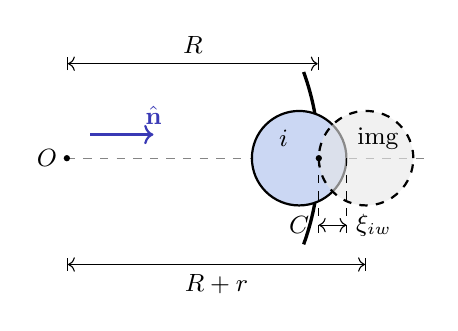
\begin{tikzpicture}[font=\small]
        \draw[very thick] (-20:3.2) arc (-20:20:3.2);
        \draw[dashed, TPNavGray] (0,0) -- (4.6,0);
        \fill (0,0) circle (0.04) node[left] {$O$};
        \draw[thick, fill=TPFresca!25] (2.95,0) circle (0.6);
        \draw[thick, dashed, fill=TPNavGray!20, fill opacity=0.6] (3.8,0) circle (0.6);
        \node at (2.75,0.25) {$i$};
        \node at (3.95,0.25) {img};
        \fill (3.2,0) circle (0.04);
        \draw[->, thick, TPBlue] (0.3,0.3) -- (1.1,0.3) node[above] {$\hat{\mathbf{n}}$};
        \draw[|<->|] (0,1.2) -- (3.2,1.2) node[midway, above] {$R$};
        \draw[dashed] (3.2,0) -- (3.2,-0.95) (3.55,0) -- (3.55,-0.95);
        \node[left] at (3.2,-0.85) {$C$};
        \draw[<->] (3.2,-0.85) -- (3.55,-0.85) node[right] {$\xi_{iw}$};
        \draw[|<->|] (0,-1.35) -- (3.8,-1.35) node[midway, below] {$R + r$};
      \end{tikzpicture}
    \end{column}
    \begin{column}{0.47\textwidth}
      % Un título por fórmula, como en «Modelo»
      \begin{itemize}
        \item \textbf{Contacto:} $|\mathbf{r}_i| > R - r$
        \item \textbf{Normal:} $\hat{\mathbf{n}} = \mathbf{r}_i/|\mathbf{r}_i|$
        \item \textbf{Imagen:} radio $r$ en $(R + r)\,\hat{\mathbf{n}}$, recalculada cada $\Delta t$
        \item \textbf{Superposición:} $\xi_{iw} = |\mathbf{r}_i| + r - R$
        \item \textbf{Fuerza:} la misma que entre partículas
        \item \textbf{Energía:} la imagen no suma; $\tfrac{1}{2}k\,\xi_{iw}^2$ se suma una vez
      \end{itemize}
    \end{column}
  \end{columns}
\end{frame}

% ---------------- SIMULACIONES ----------------
% 9
\sectiondivider{Simulaciones}

% 10 -- S05a: solo el esquema, como «Geometría del Sistema» de TP3; los valores van en «Parámetros»
\begin{frame}{Sistema 2: Geometría}
  \centering
      % E1 a escala (1 m = 4,9 cm), con x₀ = 0,24 m; Fig. 1(a) del enunciado
      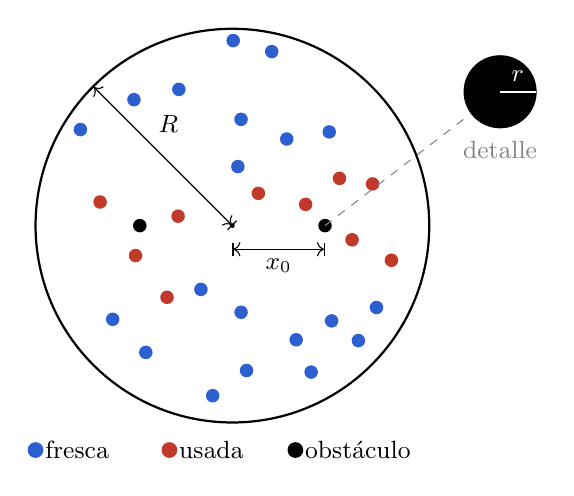
\begin{tikzpicture}[font=\small]
        \draw[thick] (0,0) circle (2.5);
        \foreach \x/\y in {0.93/0.27,-1.23/-0.38,1.52/-0.18,-0.69/0.12,-1.68/0.30,1.36/0.60,1.78/0.53,0.33/0.41,2.02/-0.44,-0.83/-0.91}
          \fill[TPUsada] (\x,\y) circle (0.0858);
        \foreach \x/\y in {-0.40/-0.81,1.23/1.19,0.69/1.10,1.26/-1.21,1.83/-1.04,-1.52/-1.19,0.07/0.75,-1.93/1.22,0.81/-1.45,1.60/-1.46,0.11/-1.10,-1.25/1.60,-1.10/-1.61,0.11/1.35,-0.68/1.73,1.00/-1.86,0.18/-1.84,0.50/2.21,-0.25/-2.16,0.01/2.35}
          \fill[TPFresca] (\x,\y) circle (0.0858);
        \fill (1.176,0) circle (0.0858) (-1.176,0) circle (0.0858);
        \fill (0,0) circle (0.03);
        \draw[|<->|] (0,0) -- node[above right, pos=0.6] {$R$} (135:2.5);
        \draw[|<->|] (0,-0.3) -- (1.176,-0.3) node[midway, below] {$x_0$};
        % detalle ampliado de un obstáculo para la cota de r
        \draw[dashed, TPNavGray] (1.176,0) -- (3.0,1.4);
        \draw[thick, fill=black] (3.4,1.7) circle (0.45);
        \draw[white, thick] (3.4,1.7) -- node[above] {$r$} (3.85,1.7);
        \node[TPNavGray, below] at (3.4,1.2) {detalle};
        % leyenda
        \fill[TPFresca] (-2.5,-2.85) circle (0.1) node[right, black] {fresca};
        \fill[TPUsada] (-0.8,-2.85) circle (0.1) node[right, black] {usada};
        \fill (0.8,-2.85) circle (0.1) node[right] {obstáculo};
      \end{tikzpicture}
\end{frame}

% 11 -- S05b (define ε_E, Nu, Fu, t₉₀, t₁₀₀, ρ, φ, realización, σ)
\begin{frame}{Sistema 2: Observables}
  \begin{databox}{Observables}
    \begin{itemize}
      \item $\varepsilon_E = \max_t |E(t)-E(0)|/E(0)$, con $t$ múltiplo de $\Delta t_2$
      \item $N_u(t)$: partículas que ya tocaron un obstáculo (usadas)
      \item $F_u(t) = N_u(t)/N$
      \item $t_{90}$, $t_{100}$: primer $t$ con $F_u \geq 0{,}9$ y con $F_u = 1$
      \item $\rho = N/(\pi R^2)$, \quad $\varphi = N r^2/R^2$
    \end{itemize}
  \end{databox}
  \par\vspace{3mm}
  \parambox{\item Realización: corrida con una semilla (posiciones y direcciones iniciales)
    \item $\langle\cdot\rangle$: media entre realizaciones; barras: $\pm\sigma$, desvío estándar muestral entre realizaciones}
\end{frame}

% 12 -- S05c: parámetros fijos y variables, con el formato de «Parámetros» de TP3 (sin rótulos 2.x;
% DEFINICIONES.md:78; D7, D8, D9, D13, D22, D33). Recibe los fijos que antes estaban en «Geometría».
\begin{frame}{Sistema 2: Parámetros}
  \small
  Parámetros de entrada fijos:
  \begin{itemize}[itemsep=1pt,topsep=2pt]
    \item $R = 0{,}51$ m; $r = 0{,}0175$ m; $m = 0{,}025$ kg; $k = 10^{4}$ N/m
    \item $v_0 = 1$ m/s, dirección $\sim U[0, 2\pi)$; $N$ sitios al azar de una red hexagonal fija
    \item $\Delta t = 10^{-5}$ s (salvo en el estudio de $\Delta t$); $\Delta t_2 = 0{,}04$ s; $t_f = 30$ s
  \end{itemize}
  Parámetros de entrada variables:
  \begin{itemize}[itemsep=1pt,topsep=2pt]
    \item Paso temporal: $\Delta t = 10^{-2}, \dots, 10^{-6}$ s ($N = 300$, sin obstáculos)
    \item Tiempo de ejecución: $N = 100, \dots, 600, 714$ ($x_0 = r$)
    \item Obstáculos: 9 valores de $x_0$ en $[r, R-r]$ ($N = 100$ y $20$; $t_{\max} = 100$ s)
    \item Distribución de rapidez: $N = 100$, sin obstáculos
    \item Densidad: $N = 25, \dots, 714$ ($x_0 = r$)
    \item Mapa: 9 valores de $x_0$ $\times$ $N = 100, \dots, 600, 700$
  \end{itemize}
  \begin{databox}{Nro.\ de realizaciones}
    \centering
    Paso: 1 \hfill Tiempo: 10 \hfill Obstáculos: 8 \hfill Rapidez: 30 \hfill Densidad: 10 \hfill Mapa: 3
  \end{databox}
\end{frame}

% ---------------- RESULTADOS ----------------
% 13
\sectiondivider{Resultados}

% 14 -- S06 (única diapositiva del Sistema 1)
\begin{frame}[c]{Sistema 1: Error Cuadrático Medio en Función de $\Delta t$}
  % Sin caja de parámetros: figura centrada a todo el ancho disponible
  \centering
  \maybeimage{figuras/F1-ecm-vs-dt.pdf}{6.9cm}{F1}
\end{frame}

% 15 -- S13a: animación de 2.3 en su propia diapositiva, como la de 2.2
\begin{frame}[c]{Sin Obstáculos --- Evolución del Sistema}
  % Corrida de generate_animations.sh: N = 100, semilla 1, sin obstáculos, t_f = 100 s
  \animacionsimple{figuras/anim-sistema2-sin-obstaculos.png}{5.1cm}{\animacionSinObstaculosURL}
  {Fotograma de la animación de 2.3}
  {\item $N = 100$}
\end{frame}

% 16 -- S10
\begin{frame}[c]{Obstáculos en $\pm x_0$ --- Evolución del Sistema}
  % Corrida de generate_animations.sh: N = 100, semilla 1, x₀ = 0,25 m, t_f = 100 s
  \animacionsimple{figuras/anim-sistema2-con-obstaculos.png}{5.1cm}{\animacionConObstaculosURL}
  {Fotograma de la animación de 2.2}
  {\item $N = 100$
    \item $x_0 = 0{,}25$ m}
\end{frame}


% 17 -- F2 principal (enunciado 2.1.a)
\begin{frame}[c]{Energía Total en Función del Tiempo}
  \resultadofigura{figuras/F2-energia-vs-t.pdf}{6.5cm}{F2}{\item $N = 300$}{}{}
\end{frame}

% 18 -- S08
\begin{frame}[c]{Error de Energía en Función de $\Delta t$}
  \resultadofigura{figuras/F3-epsE-vs-dt.pdf}{6.5cm}{F3}{\item $N = 300$
     \item $\Delta t = 10^{-5}$ s}{}{}
\end{frame}


% 19 -- S09
\begin{frame}[c]{Tiempo de Ejecución en Función de $N$}
  \resultadofigura{figuras/F4-tiempo-vs-n.pdf}{6.5cm}{F4}{\item TP4: obstáculos en $x_0 = r$
     \item TP3: sin obstáculos
     \item 10 realizaciones por $N$}{}{}
\end{frame}


% 20 -- S11
\begin{frame}[c]{Fracción Usada en el Tiempo}
  \resultadofigura{figuras/F5-fu-vs-t.pdf}{6.5cm}{F5}
    {\item $N = 100$
     \item 8 realizaciones por $x_0$}{}{}
\end{frame}

% 21 -- S12
\begin{frame}[c]{$\langle t_{90}\rangle$ en Función de $x_0$}
  % Sin caja de parámetros: figura centrada a todo el ancho disponible
  \centering
  \maybeimage{figuras/F6-t90-vs-x0.pdf}{6.9cm}{F6}
\end{frame}

% 22 -- S13z: ⟨v⟩(t) con zoom en t ≤ 3 s; define t_est (D15; figura de fedir03, b974871)
\begin{frame}[c]{Rapidez Media en el Tiempo}
  \resultadofigura{figuras/F7-v-media-vs-t-zoom-test.pdf}{6.5cm}{F7 zoom}
    {\item $N = 100$, sin obstáculos, 30 realizaciones
     \item Punteada: $t_{est} = 0{,}75$ s, inicio del estacionario
     \item Banda: $\pm\sigma$}{}{}
\end{frame}

% 23 -- S13 (usa t_est)
\begin{frame}[c]{Distribución de Rapidez en el Tiempo}
  \resultadofigura{figuras/F7b-fv-instantes.pdf}{6.5cm}{F7}
    {\item $N = 100$
     \item sin obstáculos
     \item 30 realizaciones}{}{}
\end{frame}

% 24 -- S14 (define k_BT)
\begin{frame}[c]{Distribución Estacionaria y Ajuste de Maxwell-Boltzmann}
  % Sin caja de parámetros: figura centrada a todo el ancho disponible
  \centering
  \maybeimage{figuras/F8-fv-mb.pdf}{6.9cm}{F8}
\end{frame}

% 25 -- S15 (D14, D33; datos de outputs/runtime_tp4_analisis/F9-2.4.md)
\begin{frame}[c]{$\langle F_u(30\,\mathrm{s})\rangle$ en Función de la Densidad}
  \resultadofigura{figuras/F9-fu-vs-densidad.pdf}{6.5cm}{F9}
    {\item $x_0 = r$
     \item 10 realizaciones por $N$}{}{}
\end{frame}

% 26 -- extra 2.4.b (D22; datos de outputs/runtime_tp4_analisis/F10-2.4b.md)
\begin{frame}[c]{$\langle F_u(30\,\mathrm{s})\rangle$ en Función de $x_0$ y $N$}
  % F10 (un panel, 6,3 x 3,45 in) a todo el ancho; la caja de abajo quedó vacía y se sacó
  \centering
  \maybeimage{figuras/F10-mapa-x0-n.pdf}{7cm}{F10}
\end{frame}

% ---------------- CONCLUSIONES ----------------
% 27
\sectiondivider{Conclusiones}

% 28 -- S16
% RECORDATORIOS: cada afirmación dice a qué caso se refiere; nada sobre
% el dt elegido (eso queda en 2.1.a).
\begin{frame}{Conclusiones}
  \begin{itemize}
    \item En el oscilador amortiguado, Beeman resultó el mejor esquema de integración y Euler predictor-corrector, el peor.
    \item Para sistemas con muchas partículas ($N \gtrsim 460$), la dinámica molecular regida por el paso temporal tiene mejor desempeño que la dirigida por eventos.
  \end{itemize}
\end{frame}

% 29 -- S17
\begin{frame}{Uso de IA}
  \begin{itemize}
    \item Agentes: Claude Code (Anthropic), modelo Opus 5.5 y Chat GPT (OpenAI), modelo Sol 6.1
    \item Motor: código escrito por el agente, por etapas, a partir de fórmulas verificadas por el grupo contra la presentación teórica y de las decisiones del grupo; cada etapa se revisó con sus tests antes de seguir
  \end{itemize}
\end{frame}

% 30. Cierre
\begin{frame}{}
  \vfill
  \begin{beamercolorbox}[wd=0.86\paperwidth,ht=0.72cm,dp=0.20cm,center]{frametitle}
    \LARGE Muchas gracias
  \end{beamercolorbox}
  \vspace{0.4cm}
  \begin{center}
    \maybeimage{figuras/muchas_gracias.jpeg}{3.1cm}{Insertar imagen de cierre}
  \end{center}
  \vfill
\end{frame}

% 31--32 -- S17b (D31, M5: dentro del PDF, después de "Muchas gracias" para que
% Uso de IA sea la última diapositiva de la exposición; fuente docs/ia/prompts-motor.md).
% Dos diapositivas (23/10): integradores (Sistema 1 y 2) y vecinos/grilla (CIM y TP3). Texto sin cambios.
\begin{frame}{Anexo: Prompts del Motor (1/2)}
  \small
  \textbf{Módulo TP4 y Sistema 1 · Claude Code (Opus 5.5)}\par\smallskip
  Pedido: leer el enunciado, Teórica 4 y el plan de implementación (\texttt{docs/plan/}: \texttt{DEFINICIONES.md}, \texttt{referencia/FORMULAS-VERIFICADAS.md}, \texttt{referencia/PLAN.md} y los pasos) y resumir lo entendido antes de escribir código. Después, implementar el Sistema 1 a partir de lo que el grupo ya había definido: las fórmulas de los 4 esquemas verificadas contra las diapositivas.\par\bigskip
  \textbf{Sistema 2 · Claude Code (Opus 5.5)}\par\smallskip
  Pedido: Leer el contexto. Después consultar las respuestas de la cátedra a las preguntas hechas en la clase de consultas y las decisiones del grupo (obstáculos en 2.1.b, criterio de corte de 2.1.a, energía sin la partícula imagen, grilla única, uso del CIM), y ajustar el plan a esas respuestas.\par
\end{frame}

\begin{frame}{Anexo: Prompts del Motor (2/2)}
  \small
  \textbf{CIM, grilla y N máx · Claude Code (Opus 5.5)}\par\smallskip
  Pedido: reconstrucción del TP1 al módulo TP4 \texttt{CellIndexMethod}, \texttt{NeighborFinder} y \texttt{Particle}, y revisar qué devuelve el CIM; agregar dentro del CIM el corrimiento $+R$ y la validación $|r| \leq R$; escribir el script que mide el N máximo con la grilla (cuadrada y hexagonal); escribir el test CIM contra fuerza bruta con la misma semilla. Explicar todo el código aplicado.\par\bigskip
  \textbf{Grilla del TP3 y medición de tiempos · Claude Code (Opus 5.5)}\par\smallskip
  Pedido: leer el generador de escenarios del TP3 (\texttt{StageGeneration} y lo que lo usa) y proponer un plan para que el TP3 genere la condición inicial con la misma grilla que el TP4 (\texttt{GridPlacement}: hexagonal) y volver a correr el TP3. Condiciones: pedir confirmación antes de tocar código del TP3 que no sea el generador; corrida por tandas y reanudable; salidas fuera del repo o ignoradas por git.\par
\end{frame}

\end{document}
